\section{Bubble Sort}
\label{sec:bubble_sort_teo}

O Bubble Sort, também conhecido como "Ordenação por bolha" ou "Ordenação por flutuação", é um dos algoritmos de ordenação mais simples.

Neste algoritmo, são realizadas comparações entre os dados armazenados em um vetor de tamanho \( n \). Cada elemento na posição \( i \) é comparado com o elemento na posição \( i+1 \). Quando a ordenação procurada — seja ela crescente ou decrescente — é encontrada, ocorre uma troca de posições entre os elementos.

O algoritmo executa dois laços principais:

\begin{enumerate}
	\item[\textbf{1.}] O primeiro laço percorre a quantidade de elementos do vetor:
	      \begin{verbatim}
    for (j = 1; j <= n; j++)
    \end{verbatim}

	\item[\textbf{2.}] O segundo laço, que está dentro do primeiro, percorre da primeira à penúltima posição do vetor:
	      \begin{verbatim}
    for (i = 0; i < n - 1; i++)
    \end{verbatim}
\end{enumerate}


\begin{figure}[!ht]
	\centering
	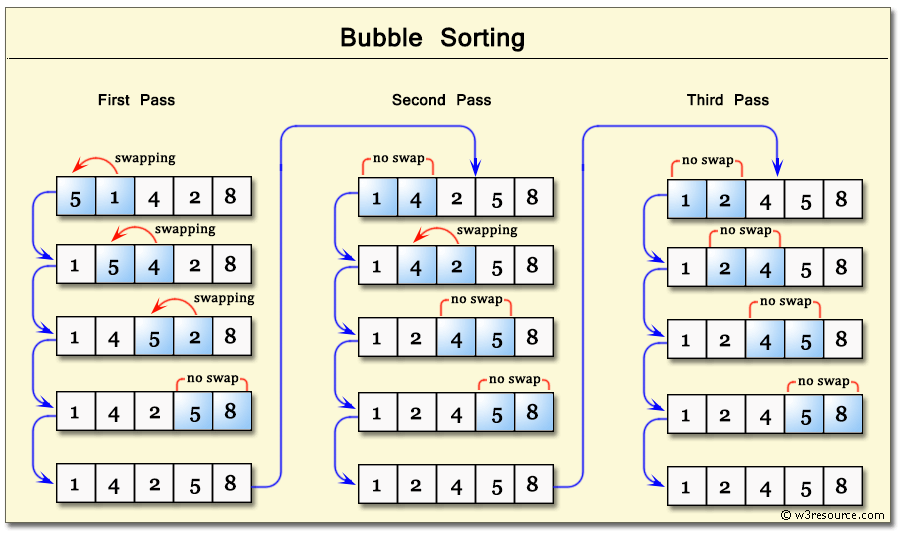
\includegraphics[scale=0.3]{figures/bubble/bubbleDiagram.png}
	\caption{Diagrama exemplo de um Bubble Sort}
	\label{fig:bubble_sort_example}
\end{figure}


\FloatBarrier

\newpage

\subsection{Bubble Sort Iterativo}

\begin{algorithm}
	\caption{Bubble Sort}
	\label{algo:bubble_sort_it}
	\begin{algorithmic}[1]
		\Require{Lista $A = A_1, A_2, \ldots, A_n$}
		\Ensure{Lista $A$ ordenada}
		\Statex
		\Function{BubbleSort}{$A$}
		\For{$j \gets 1$ to $n - 1$}
		\For{$i \gets 0$ to $n - 2$}
		\If{$A[i] > A[i + 1]$}
		\State $aux \gets A[i]$
		\State $A[i] \gets A[i + 1]$
		\State $A[i + 1] \gets aux$
		\EndIf
		\EndFor
		\EndFor
		\EndFunction
	\end{algorithmic}
\end{algorithm}

\subsubsection{Análise}
Nesse algoritmo, o fator relevante que determina o seu tempo de execução é o número de comparações realizadas. Considerando que o algoritmo foi implementado para um vetor com \( n \) posições, o número de iterações do primeiro laço é \( n \).

O segundo laço possui \( n-1 \) iterações, mas como ele está interno ao primeiro, ele será executado \( n(n-1) = n^2 - n \) vezes. Portanto, podemos dizer que o tempo de execução do algoritmo Bubble Sort, em sua forma iterativa, será \( O(n^2) \), pois:

\[
	\lim_{n \rightarrow \infty} \frac{n^2 - n}{n^2} =
	\lim_{n \rightarrow \infty} \frac{n - 1}{n} =
	\lim_{n \rightarrow \infty} 1-\frac{1}{n} =
	1 \in \mathbb{R}^*_+.
\]

De forma análoga, podemos dizer que o Bubble Sort será \( \Omega(n^2) \) e \( \Theta(n^2) \).

Nesse algoritmo, não há situações melhores ou piores. O comportamento do algoritmo não mudará, independentemente do valor de entrada. Ele realizará todas as comparações, mesmo que desnecessárias.

\newpage

\subsection{Bubble Sort Recursivo}

\begin{algorithm}
	\caption{Bubble Sort Recursivo}
	\label{algo:bubble_sort_recursivo}
	\begin{algorithmic}[1]
		\Require{Lista $A = A_1, A_2, \ldots, A_n$}
		\Ensure{Lista $A$ ordenada}
		\Statex
		\Function{BubbleSortRecursivo}{$A, n$}
		\If{$n == 1$}
		\Return{}
		\EndIf
		\For{$j \gets 0$ to $n - 1$}
		\If{$A[j] > A[j + 1]$}
		\State $aux \gets A[j]$
		\State $A[j] \gets A[j + 1]$
		\State $A[j + 1] \gets aux$
		\EndIf
		\EndFor
		\State \Call{BubbleSortRecursivo}{$A, n - 1$}
		\EndFunction
	\end{algorithmic}
\end{algorithm}

\subsubsection{Análise}
Agora, faremos a análise da complexidade da versão recursiva do algoritmo Bubble Sort, utilizando os quatro métodos estudados na disciplina:

\begin{enumerate}
	\item \textbf{Substituição:}

	      Com esse método, mostraremos, por indução, que \( T(n) = T(n-1) + n \) é limitada por \( f(n) = n^2 \).

	      \begin{itemize}
		      \item \textbf{Caso base:} \( n = 1 \).

		            Sabemos que \( T(1) = 1 \) e \( f(1) = 1 \).

		            Logo, \( T(1) \leq f(1) \).

		            Portanto, a base da indução é válida.

		      \item \textbf{Hipótese de Indução:} Suponha que \( T(k) \leq k^2 \) para todo \( 1 < k \leq n \).

		      \item \textbf{Passo indutivo:} Queremos provar que \( T(n+1) \leq (n+1)^2 \).

		            Observe que:
		            \begin{align*}
			             & T(n) \leq n^2                                  &  & \text{(pela hipótese de indução)} \\
			             & \Longrightarrow T(n) + n \leq n^2 + 2n         &  & \text{(pois \( n \leq 2n \))}     \\
			             & \Longrightarrow T(n) + n \leq n^2 + 2n         &  & \text{(pois \( n \leq 2n \))}     \\
			             & \Longrightarrow T(n) + n + 1 \leq n^2 + 2n + 1                                        \\
			             & \Longrightarrow T(n+1) \leq (n+1)^2
		            \end{align*}
	      \end{itemize}

	      Portanto, para todo \( k \) tal que \( 1 < k \leq n \), \( T(n) \leq f(n) = n^2 \).

	      Assim, \( T(n) \) é \( O(n^2) \).

	\item \textbf{Método Mestre:}

	      Esse método permite resolver recorrências da forma \( T(n) = a \, T\left(\frac{n}{b}\right) + \Theta(n^k) \), com \( a \geq 1 \), \( b > 1 \), e \( k \geq 0 \), onde \( a \), \( b \), e \( k \) são constantes.

	      Como não é possível escrever \( T(n) = T(n-1) + n \) nesse formato, sem que \( b \) seja uma função de \( n \), não podemos aplicar o Método Mestre a essa recorrência.


	\item \textbf{Árvore Recursiva:}

	      Esse método consiste em desenhar uma árvore cujos nós representam os tamanhos dos problemas correspondentes. Cada nível \( i \) contém todos os subproblemas de profundidade \( i \). Dois aspectos importantes devem ser considerados: a altura da árvore e o número de passos executados em cada nível. A solução da recorrência, que é o tempo de execução do algoritmo, é a soma de todos os passos de todos os níveis:
	      \[
		      \sum_{i=0}^{\text{niveis}} (\text{tempo por nó}) \cdot (\text{quantidade de nós})
	      \]
	      Precisamos saber a quantidade de níveis, ou seja, o valor que corresponde à altura da árvore recursiva. Nesse caso, temos a seguinte árvore recursiva:

	      \[\begin{tikzcd}
			      {T(n)} \\
			      {T(n-1)} \\
			      {T(n-2)} \\
			      {T(n-3)} \\
			      {T(n-i)}
			      \arrow[from=1-1, to=2-1]
			      \arrow[from=2-1, to=3-1]
			      \arrow[from=3-1, to=4-1]
			      \arrow[from=4-1, to=5-1]
		      \end{tikzcd}\]

	      A partir da árvore de recorrência, podemos formar a seguinte tabela:

	      \begin{table}[h!]
		      \centering
		      \begin{tabular}{lrrr}
			      \toprule
			      Nível da Árvore & Tamanho da Entrada & Custo por Nó & Quantidade de Nós \\
			      \midrule
			      0               & \( n \)            & \( n \)      & 1                 \\
			      1               & \( n-1 \)          & \( n-1 \)    & 1                 \\
			      2               & \( n-2 \)          & \( n-2 \)    & 1                 \\
			      3               & \( n-3 \)          & \( n-3 \)    & 1                 \\
			      \vdots          & \vdots             & \vdots       & \vdots            \\
			      \( i \)         & \( n-i \)          & \( n-i \)    & 1                 \\
			      \bottomrule
		      \end{tabular}
	      \end{table}

	      \FloatBarrier

	      Com isso, podemos concluir que a soma de todos os passos executados por todos os níveis é dada por:
	      \[
		      T(n) = 1 + 2 + 3 + \ldots + (n - 2) + (n - 1) + n = \frac{(n + 1) n}{2} = \frac{n^2 + n}{2}
	      \]

	      Portanto, temos:
	      \[
		      T(n) = O(n^2)
	      \]

	\item \textbf{Iteração:}

	      Aqui, expandiremos a recorrência até o caso base.
	      \begin{align*}
		      T(n) & = T(n-1) + n                                               \\
		           & = T(n-2) + (n - 1) + n                                     \\
		           & = T(n-3) + (n - 2) + (n - 1) + n                           \\
		           & \vdots                                                     \\
		           & = T(n-i) + (n - i + 1) + (n - i + 2) + \dots + (n - 1) + n
	      \end{align*}

	      O caso base ocorrerá quando \( i = n - 1 \). Nesse momento, teremos:

	      \[
		      T(n) = T(1) + 2 + 3 + \dots + (n - 1) + n
	      \]

	      A soma \( 2 + 3 + \dots + n \) é uma progressão aritmética, e pode ser calculada por:

	      \[
		      T(n) = T(1) + \frac{(2 + n)(n - 1)}{2}
	      \]

	      Assim, substituindo \( T(1) \) por uma constante \( c \), obtemos:

	      \[
		      T(n) = c + \frac{n^2 + n - 2}{2}
	      \]

	      Como \( c \) é uma constante, podemos ignorá-la na análise assintótica e dizer que:

	      \[
		      T(n) = O(n^2)
	      \]


\end{enumerate}







